%--------------------------------Dependencies----------------------------------%
%   tikz                                                                       %
%-------------------------------Main Document----------------------------------%
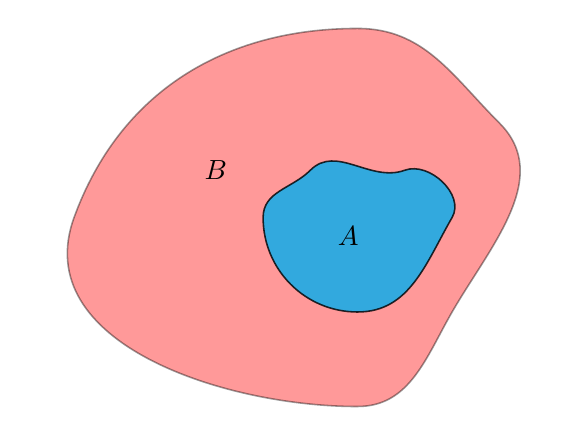
\begin{tikzpicture}[line width=0.2mm, scale=1.2]

    % Coordinates for the bigger blob.
    \coordinate (P1) at ( 0.0, -2.0);
    \coordinate (P2) at ( 1.0, -1.0);
    \coordinate (P3) at ( 1.5,  1.0);
    \coordinate (P4) at ( 0.0,  2.0);
    \coordinate (P5) at (-3.0,  0.0);

    % Coordinates for the inner blob.
    \coordinate (Q1) at ( 0.0, -1.0);
    \coordinate (Q2) at ( 1.0,  0.0);
    \coordinate (Q3) at ( 0.5,  0.5);
    \coordinate (Q4) at (-0.5,  0.5);
    \coordinate (Q5) at (-1.0,  0.0);

    % Coordindates to label things.
    \coordinate (A) at (-0.1, -0.2);
    \coordinate (B) at (-1.5,  0.5);

    % Draw the bigger blob.
    \draw[fill=red, opacity=0.4] (P1) to [out=0,    in=-120] (P2)
                                      to [out=60,   in=-45]  (P3)
                                      to [out=135,  in=0]    (P4)
                                      to [out=-180, in=70]   (P5)
                                      to [out=-110, in=-180] cycle;

    % Draw the inner blob.
    \draw[fill=cyan, opacity=0.8] (Q1) to [out=0,    in=-120]  (Q2)
                                       to [out=60,   in=20]    (Q3)
                                       to [out=-160, in=45]    (Q4)
                                       to [out=-135, in=90]    (Q5)
                                       to [out=-90,  in=180]   cycle;

    % Labels for the two blobs.
    \node at (A) {$A$};
    \node at (B) {$B$};
\end{tikzpicture}
